\documentclass[twoside]{wiss}

\usepackage{graphicx}
\usepackage{nidanfloat} %% appended in WISS2010 for Future Vision (2010/7/7:akita)
\usepackage{multicol}
\usepackage{here} % [H]とするとその場所に配置されるらしい

%% balance.styを追加 (2012/9/27:watanabe, Igarashi)
\usepackage{balance}    %% 最後のページの高さを揃えるために追加  (2012/9/27:watanabe, Igarashi)
%%% 最後のページの2段組の高さを揃える.\balanceを入れる.
%%% そろえたくないときは,\nobalance

\long\def\comment#1{}

% \journalhead{{\EP}: Password Management based on Episodic Memories}
\journalhead{「超」ナビゲーション}

\begin{document}

\title{「超」ナビゲーション}
\etitle{} %2012年では英文タイトルは廃止されました.記入しないでください
% Supernavigation

\author{増井 俊之\affil{Toshiyuki Masui, 慶應義塾大学 環境情報学部}}

\begin{abstract}
単純な装置で大規模な階層データを効率的にナビゲーションする手法を提案する。

ファイルシステムや住所のような大規模な階層データから項目を選ぶ場合、
% 階層を上下に移動したり同じ階層内の選択項目を移動したりするのが普通である。
階層の上下移動や同一階層内の選択項目移動を組み合わせるのが普通である。
例えば日本の全住所リストから「神奈川県藤沢市遠藤」を検索する場合、
都道府県リストから神奈川県を選択し、神奈川県の市町村リストから藤沢市を選択し、...
といった操作を繰り返す。
別の県や市町村の住所を選択する場合は上位階層に移動してから同様の操作を行なう。
このようなナビゲーションを行なうためには
階層を上下移動する手法と
階層内を移動する手法が必要になるため、
4個以上のキーが用いられることが多い。

本論文では、2個のキーだけを使ってこのような階層データ内ナビゲーションを実現する
手法「Gear」を提案する。
Gearは以下のふたつの

\begin{enumerate}
\item 階層内の項目選択時に端まで来た場合は上の階層に移動する
\item 選択中の項目に下位階層がある場合は一定時間後に下の階層に移動する
\end{enumerate}

これらの工夫により、2個のキーだけであらゆる階層データを効率的にナビゲーションする
ことが可能になる。
キー以外の様々な入力デバイスを利用することができる。
\end{abstract}

\maketitle

\section{はじめに}

大量のデータを扱うために階層的に整理する手法がよく利用されている。

計算機のファイルシステム、住所、ISBN(書籍情報)、JANコードなど、
大規模なデータの多くは階層構造として表現されている。

Unixで導入された階層型ディレクトリは現在あらゆるパソコンで導入されている。

階層型ファイルシステムはUnixで導入されたものであるが、
現在は他のOSでも標準的になっており、
全世界のデータを表現するURLでも...

URL、ファイル名、住所のような大規模データは木構造で表現されることが多い。

住所データのように本質的に階層的なものもあるし
URLやパソコンのファイル名は階層的な名前を持っているし、
世の中の多くの情報は階層的な構造を持っており、

写真も日付により階層構造である

(図を描く)

大規模な木構造の中のノードを検索する手法が重要である。
情報視覚化を利用して
GUIを用いる方法も多数提案されているが
\cite{Johnson:1991:TSA:949607.949654},
  Treemapとか
パソコンや携帯機器では
シンプルなキー操作を利用する手法も広く使われている。

例えばMacのFinderでは、
Macのファインダではファイルの階層構造を視覚化/ナビゲーションするために
複数の手法が用意されており、
単純なマウス/キー操作でナビゲーションを行なうことができるようになっている。
...みたいなキー操作で階層情報をたどることができる。

木構造のノードをたどることによって
そこから必要な情報を取得するための様々な手法が利用されている。

(手法)

パソコンや携帯機器のキーやボタンを利用して木構造のナビゲーションを行なう場合、
木構造の上下、兄弟を移動することで目的の情報にたどりつくのが普通である
大抵は上下/左右のキーなどを利用する

(ここを図解説明する)

たとえばFinderでは... AppleRemoteでは...

(提案)

このような手法でナビゲーションを行なうには、3個以上のスイッチが必要になる。

昔の携帯電話などに登載されていたジョグダイヤルでは
上下方向の回転の他にダイヤルを押す操作で
項目を選択したり下の階層に移動したりするようになっていたし、
AppleRemoteやTV付属のリモコンでは4方向のキーでナビゲーションを行なうようになっている。

階層情報のナビゲーションを2個のスイッチだけで実行することができれば、
非常に単純な装置と操作だけでナビゲーションが可能になるため、
広い範囲で利用できるようになるはずである。

本論文では、2個のスイッチだけで階層構造を効率的にナビゲーションする装置「Gear」について述べる。

これらの装置を総称して「Gear」と呼ぶことにする。

Gearでは、▲と▼というふたつのキーのみを利用して階層データのナビゲーションを行なう。

\section{Gearの説明と利用例}

▲と▼

(1) 階層内の項目選択時に端まで来た場合は上の階層に移動する
(2) 選択中の項目に下位階層がある場合は一定時間後に下の階層に移動する

Macのファインダを利用してGearの動きを説明する。

以下のような階層構造をもつファイルシステムのナビゲーションを考える。

\begin{figure}[H]
\centerline{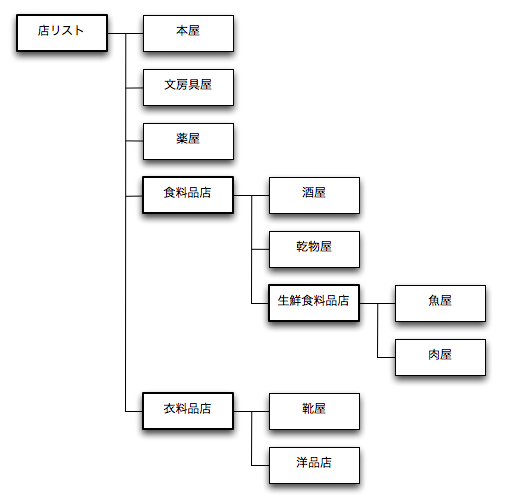
\includegraphics[width=60mm,bb=0 0 509 502]{figures/ae9216b00626f9c4eea44cc380f25886.png}}
\caption{ssss}
\label{screenshot}
\end{figure}

\subsection*{Macのファインダ上での階層情報ナビゲーション}

Macのファインダでは▲▼◀▶という4個のキーでファイルシステムのナビゲーションを行なうことができる。

「店リスト」をMacのファインダで表示して「本屋」を選択すると
表示は以下のようになる。

\begin{figure}[H]
\centerline{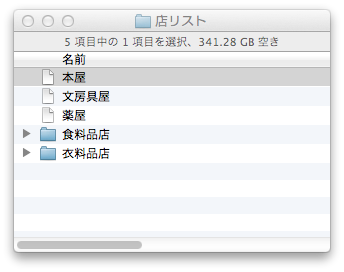
\includegraphics[width=60mm,bb=0 0 344 272]{figures/9b121bec45e5b480e5ac64fdd0f82592.png}}
\caption{ssss}
\label{screenshot}
\end{figure}

ここで▼を押すと

\begin{figure}[H]
\centerline{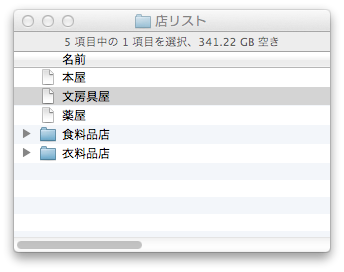
\includegraphics[width=60mm,bb=0 0 344 272]{figures/f43016d1b524baf414f2c32c48fe9588.png}}
\caption{ssss}
\label{screenshot}
\end{figure}

さらに二回▼を押すと、以下のように「食料品店」が選択される。

\begin{figure}[H]
\centerline{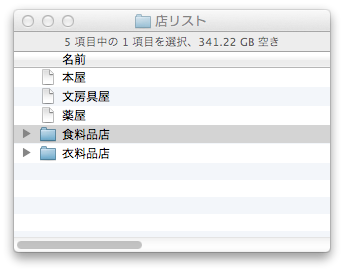
\includegraphics[width=60mm,bb=0 0 344 272]{figures/c074cd6daec3da0341125d1492b8a09c.png}}
\caption{ssss}
\label{screenshot}
\end{figure}

「食料品店」は下位階層を持っており、
ここで▶キーを押すことによって以下のように下位階層が表示される。

\begin{figure}[H]
\centerline{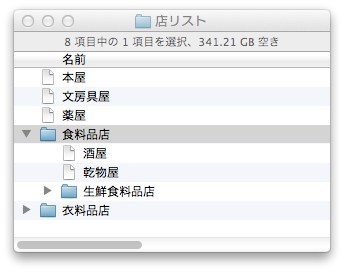
\includegraphics[width=60mm,bb=0 0 344 272]{figures/51d867d4721f65c18e84172c8818e137.png}}
\caption{ssss}
\label{screenshot}
\end{figure}

ここで▼キーを押すことによって「酒屋」を選択したり、
「生鮮食料品店」を選択してから▶を押してさらに下位階層を
表示することができる。

\begin{figure}[H]
\centerline{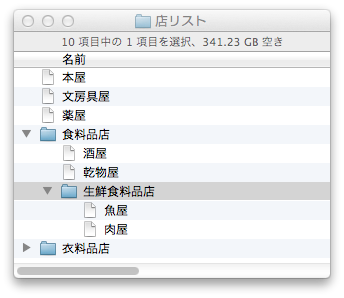
\includegraphics[width=60mm,bb=0 0 344 298]{figures/ce3ee682612de44d6c663a7323c262a6.png}}
\caption{ssss}
\label{screenshot}
\end{figure}

また、この状態で◀キーを押すと下位層の表示を消し、
もとの状態に戻すことができる。

以上のように、Macのファインダでは4個のキーを使って
階層データのナビゲーションを行なうことができる。
リモコンその他でも同様の手法が利用されている。

□ Gearによる階層データのナビゲーション

Gearでは▲と▼だけを利用してナビゲーションを行なうことができる。

Gearで「店リスト」を表示すると以下のようになる点は同じであるが、
▼を3回押して「食料品店」を選択したまま一定時間放置すると、
「食料品店」の下位層が自動的に展開され、
その最初の要素が選択される。

\begin{figure}[H]
\centerline{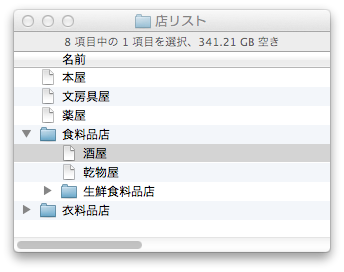
\includegraphics[width=60mm,bb=0 0 344 272]{figures/2387e402f81dbe7917e04df82b0a659c.png}}
\caption{ssss}
\label{screenshot}
\end{figure}

同様に、 ここで▼を2回押して「生鮮食料品店」を選択したまま一定時間放置すると、
「食料品店」の下位層が自動的に展開され、
その最初の要素が選択される。

\begin{figure}[H]
\centerline{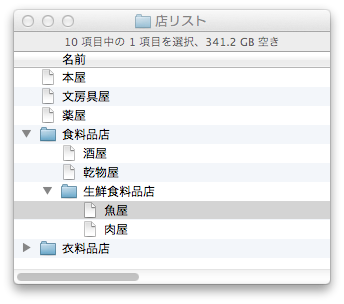
\includegraphics[width=60mm,bb=0 0 344 304]{figures/1b1955309d3baefda8e1b614cf06df62.png}}
\caption{ssss}
\label{screenshot}
\end{figure}



食料品店を選択した状態から放置せずにすぐに▼を押すと、
下位層は展開されず、次の「衣料品店」が選択される。

\begin{figure}[H]
\centerline{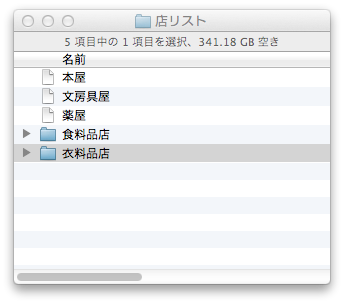
\includegraphics[width=60mm,bb=0 0 344 304]{figures/c5c757d8f79d5a8a9c85eef25600ba66.png}}
\caption{ssss}
\label{screenshot}
\end{figure}

ここで放置すると下位層が自動的に展開されて
「靴屋」が選択される。

\begin{figure}[H]
\centerline{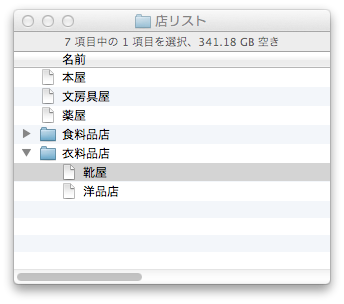
\includegraphics[width=60mm,bb=0 0 344 304]{figures/fddd5777d39924ea3f0220ae39a604c1.png}}
\caption{ssss}
\label{screenshot}
\end{figure}



XXXXの状態から▲キーを押すと、
下位層は自動的に閉じられてYYYYの状態に戻る。 
さらに▲キーを押すと
「食料品店」の下位の層も閉じられ、ZZZZの状態になる。

このように、

(1)下位層が存在するときキー入力を行なわずに放置すると下位層が自動的に展開される
(2)リストの端でさらに▲▼キーを押すと下位層は閉じられる

という方針により、
▲と▼のふたつのキーだけで
階層データをナビゲーションすることが可能になる。


\section{議論}

\subsection*{音声を利用したナビゲーション}

\subsection*{木構造しか使えないのでは?}

辞書のようなデータは読みや綴りで階層的に分類できるし、
時刻情報のような連続的なものでも
年/月/日/時間/分/秒のような階層で表現することができるので

辞書のようなフラットなデータや時刻のような連続的なデータも
読みなどを利用して階層的に表現可能であるし、
SNSの友達関係のようなネットワーク構造も
木構造的に表現することは可能なので、
ほぼあらゆるデータは木構造で表現可能だといえる。

\subsection*{誰が使うのか}

  はっきり言って、ほとんど誰でも使えると思う

  Unixでよく使うコマンドは cd, ls, more とかである
  FinderとかExplorerとかの基本ソフトで使う
  これ以外にはキーワード検索とかもあるけど

\subsection*{ザッピング}
   受動的な人でも楽しめるということ

  決定ボタンを押す方式だと、単に回転するだけでは次のページに移ることができない

\subsection*{操作が超シンプルだというのはどういうことか}

  かなりの運動障害があっても使える
  操作が少ないので、誰でも試行錯誤でなんとかなるだろう
  一方、筆者は毎日食卓からGearを使ってニュースを見たり音楽を聞いたりしている
  障害があってもなくても同じように便利だというのが理想である

\subsection*{テレビとWebの融合が失敗した理由}
   そもそも姿勢が違うのである
   前かがみになって入力装置を操作するのはテレビには向いいない

\subsection*{ひとつの階層に沢山のデータを置いてはいけない。スクロールの速度にもよるが、20個以下程度が妥当と思われる。}
   読みの場合は「あ」「か」「さ」

\subsection*{どれぐらい大きなデータに使えるか}

   普通にあらゆるデータに使えるといえるだろう
   10レベルで6階層あれば10\^6のコンテンツに対応できるとか

\subsection*{どういうデータに使えるか}
   Gearは木構造にしか適用できない
   専門的に管理されているデータは木構造が多く、
   そうでないものはタグなどを利用してネットワーク構造にするのが良いと思われる
   あらゆるネットワーク構造は木構造に変換可能だし
     表型式でも木構造の一種と考えることができる
     Cでは「配列の配列」が「表」だが
   同じデータがあちこちに出てきてもよい
     日付による分類とキーワードによる分類

\subsection*{ザッピングについて}
   下矢印だけで次頁に移動できる!
   最下位の層でザッピングできる
   単に「次」を押していけば漫画や順番に
   「前」の場合はそうはならないが、「次」の方が圧倒的に多いはずだから大丈夫

\subsection*{どういうデバイスを使うか}
  「次」「前」だけでいいから2個のスイッチだけでよい
   圧力センサやローラーなど、各週の実装が可能である
   (写真いろいろ)

\subsection*{障害対応}

「障害者」用の装置を作っては駄目で、障害が有ってもなくても使える装置を作るべきだろう。

同様に、初心者用/老人用/子供用のシステムを作るよりも、初心者でも老人で
も子供でも使えるシステムを作る方がスジが良いと思う。

\subsection*{時間を使うことはどうなのか}

ALS用文字入力システムではタイミングで選択操作を行なっている
  何と呼ぶのだっけ?
  腕は自由に動かないが、あるタイミングで腕を動かすことは可能だというタイプの障害が存在し、
    そういう症状は多い
e.g. Pete

\subsection*{選択以外の操作}

普通のWebページだとスクロール操作が必要になるが
  スクロールはなんとか大丈夫
  早送りとかは工夫が必要
    だけどできる
音量や画面の明るさ調整などは別操作が必要になるだろう
     これは別のチャンネルを利用すべきかもしれない
     別になっている方が一般に望ましいだろう
       だからiPhoneでもAndroidでも音量だけは別操作になっていてメニューで選んだりしない

\subsection*{速度について}
   もちろんパソコン上の操作より遅い
   装置が簡単だということがメリットだろう
     トレードオフである
   マウスが使える状況では無理にGearを使う必要などないだろう
     ズーミングでもなんでも使えばいい

\subsection*{手法の新規性について}

Gearを開発してから
9ヶ月にわたって何十人もの研究者や開発者に意見/感想を求めているが、
Gearと同じ手法の存在は確認できていない。

手法が単純であり、
一度使い方を知ってしまえば問題なく使えることは確認できている。

\subsection*{実装}

Linda?
2
\section{結論}

{\scriptsize
\bibliographystyle{jwiss}
\bibliography{paper}
}

\end{document}



